\documentclass[a4paper,english,pointlessnumbers,bibtotoc,BCOR1.5cm,headsepline,DIV12,appendixprefix,final,openany]{scrbook}

\usepackage[english]{babel}
\usepackage[utf8]{inputenc}
\usepackage{lmodern}
\usepackage[T1]{fontenc}
\usepackage{graphicx}
\usepackage{caption}
\usepackage[hidelinks]{hyperref}
\usepackage{bibgerm}
\usepackage{url}
\usepackage{svg}

\graphicspath{ {./images/} }

\setlength{\parindent}{0em} 

\begin{document}

\frontmatter
\subject{{\LARGE Großer Beleg}}
\title{Software-defined CPU modes}
\author{Pascal Stöver}
\publishers{Technische Universität Dresden\\
Fakultät Informatik\\
Institut für Systemarchitektur\\
Professur Betriebssysteme
\begin{minipage}{\textwidth}%\\
    \vskip 6cm
     {\normalsize }\begin{tabular}{ll}
    Betreuender Mitarbeiter: &
    Dr.-Ing. Michael Roitzsch\tabularnewline
    Betreuender Mitarbeiter:&
    Dr.-Ing. Nils Asmussen\tabularnewline
    \end{tabular} {\normalsize }\end{minipage}}

\maketitle

\tableofcontents
\listoffigures

\mainmatter

\chapter{Introduction}
\pagenumbering{arabic}
In the past, the interaction between the operating system and the processor was
relatively straightforward. A privileged mode, known as the kernel mode, granted
access to privileged features such as page table manipulation and interrupt
handling. This mode hosted the operating system, overseeing applications in the
unprivileged user mode. However, in recent years, the operating systems and
security communities have sought more than these two simplistic modes to enhance
performance and security. In response to this demand, hardware manufacturers introduced a variety of
new modes, addressing aspects like nested paging for hypervisors or modes
designed for heightened isolation, providing an exceptionally secure context for
execution. While these modes offer solutions for various specialized use cases,
they also introduce significant complexity to hardware, incurring substantial
development costs. As ideas for new modes continue to emerge, a crucial question
arises: Is it feasible to abstract the intricate mode-handling hardware into
software, thereby enabling software-defined CPU modes?\par 
Constructing a prototype of a CPU equipped with software-defined modes poses two
significant challenges. Firstly, there is the issue of handling a mode switch in
software without incurring a significant performance overhead. Secondly, the design of
a memory protection mechanism needs to address the complexity of accommodating
an arbitrary number of modes. The current paging mechanism, designed with only two
modes in mind, is optimized for this specific use case and falls short of
providing the required performance to handle a substantial number of modes, due
to a inefficient handling of access rights for multiple modes which is done on a
three bit per mode level. Consequently, a novel approach to memory protection
must be devised, one that transcends the limitations of the existing mechanism and allows for the dynamic
management of an extensive range of modes. The resolution of these challenges is
pivotal in realizing a functional prototype that not only supports
software-defined CPU modes effectively but also addresses the associated
performance considerations and memory protection requirements.\par
Previous efforts, particularly the work of von Elm.\cite{Cve}, have delved into addressing
the two aforementioned challenges. Von Elm's work, while successfully
implementing a mode switch mechanism with multiple definable modes, placed a
greater emphasis on devising a memory protection mechanism suitable for
accommodating multiple modes. In focusing on this aspect, he developed a
highly efficient protection mechanism that leverages a combination of paging and
segmentation to meet the required specifications. However, it's essential to
note that the actual mode switch, despite the advancements in memory protection,
remains hardware-based in his implementation.To simplify the hardware
implementation, von Elm opted for a hierarchy-based approach, necessitating a
predefined supervisor mode. While effective in certain respects, this
hierarchical approach falls short of providing the flexibility inherent in a
fully software-based mode switch behavior.\par
In this study, I leverage von Elm's approach for memory protection but overhaul
the implementation of mode switching behavior, which is currently predominantly
hardware-based. I aim to make the switch behavior entirely definable in
software, introducing the concept of independent modes that can be dynamically
created and utilized during runtime. To achieve this, I introduce a novel mode
named the \emph{Mode Switch Mode}. This mode comes into play whenever a mode switch
is required and dictates the alterations to crucial registers necessary for the
transition. Adopting a design incorporating this mode empowers programmers to
write the code responsible for executing the actual mode switch. As an
alternative approach, the Mode Switch Mode is offloaded to a secondary CPU known
as the \emph{Control Core}. This dedicated CPU activates each time a mode switch
occurs and, based on its own programming, changes the mode of the main CPU. The
goal is to alleviate concerns about altering the CPU state for the code running
on the Control Core, thereby reducing the state-save overhead. While some
benchmarks demonstrate a performance gain, the limited scope of these
microbenchmarks and the absence of evaluation of hardware costs provide only
suggestive evidence rather than conclusive statements regarding the comparison
of the two approaches. Consequently, this thesis primarily underscores the
feasibility of software-defined CPU modes through prototypical implementations
of the two proposed designs.\par
This thesis is organized as follows: Chapter 2 provides an exploration of
preexisting mode isolation techniques, along with general information about CPU
architecture, with a focus on the Risc-V architecture, which serves as the
framework for my designs. The gem5 simulator is introduced as the primary tool
employed for the simulation of my designs. In Chapter 3, a comprehensive
overview of von Elm's work, which forms the basis of this thesis, is presented.
Chapter 4 delves into the detailed presentation of the two designs, discussing
various design choices. The subsequent chapter, Chapter 5, offers an insight
into the implementation of these designs within the gem5 simulator. Moving on to
Chapter 6, the microbenchmarks are explained, and the results of these
benchmarks are evaluated. Limitations of the benchmarks are also revealed in
this section. In Chapter 7, a more in-depth examination of these shortcomings is
provided, accompanied by an overview of potential avenues for future
improvements to mitigate these issues. Finally, Chapter 8 concludes the thesis,
offering a concise description of the contributions made in the course of this
research.
\chapter{Background}

Before presenting the design and implementation of a new approach to CPU modes this chapter
will give some background information about CPU modes, their definition and how
they are used currently. This section will also give a brief explanation
of the RISC-V architecture and the gem5 simulator, which are later used to implement
and simulate some of the designs. 

\section{CPU Modes}
In the dynamic world of computing, the central processing unit (CPU) is the core
of any digital system. An essential aspect of modern CPUs is the distinction
between operating modes. These modes play a critical role in efficient resource
management, enabling multitasking, and enhancing security in today's computing
systems.\par
While the most well-known examples of these modes are user and kernel mode,
recent years have witnessed the emergence of additional modes tailored to
specific scenarios. These include Hypervisor modes to facilitate
hardware-supported virtualization, monitor modes to establish isolated security
contexts, and more. Manufacturers like Intel (with technologies such as SGX and
MPK) and ARM (with TrustZone) have already incorporated these modes into their
CPUs. Given this evolving landscape, there is a need for a broader understanding
of modes and mode switches.\par
To grasp the concept of modes, it's essential to first comprehend how a CPU
executes software at an abstract level. Imagine a CPU as a canvas, and all
software that runs on it is represented by an instruction stream. This stream is
consumed and interpreted by the CPU, effectively programming it. Throughout this
process, internal components like Arithmetic Logic Units (ALUs) and load-store
units are invoked, leading to changes in the CPU's state. These changes can be
seen as the execution of a program. Roitzsch et al.\cite{Roitzsch} refer to this part of the
CPU as the ``data plane" since it influences the program's state in memory.
A set of execution semantics, definied by the behaviour of the components in the
data plane, can be seen as a mode.\par
The paper introduce another component called the ``control plane", which represents
the logic governing how the CPU modifies the program's state in memory. Unlike the
modular building blocks in the data plane, the control plane tends to be
complex, and hardwired. A mode switch, represented by the control plane,
signifies a stateful transition to the semantics of the data plane. These
semantics can vary in their impact on the system, with access to more robust
semantics often considered a privilege. Consequently, modes are sometimes
referred to as privilege levels, and mode switches are termed privilege
elevation. In the following sections, I will illustrate this definition with
examples, exploring Memory Protection Keys, x86 protection rings, and ARM's TrustZone,
applying this concept at various levels of abstraction, from minor memory
protections to comprehensive system-level transformations.\par

\subsection{Memory Protection Keys}
Memory Protection Keys (MPK) represent a notable feature available in x86
processors. When activated, MPK leverages four previously unused bits within
each page-table entry to encode one of sixteen keys. Each page can be tagged
with one of these keys. By setting the "write disable" bit for a particular key,
all attempts to write to a page with that key value are blocked, and setting the
"access disable" bit also prevents reads \cite{Corbet}. These keys can be assigned to
different threads, and if a thread attempts to access a page with a mismatched
key, it triggers a segmentation fault. To modify permissions for various pages,
only the permissions associated with the corresponding key need to be changed.
Such changes can be done by everyone which means that MPK can only be used to
protect against mistakes and not againgst attacks. This approach saves us from
the overhead of altering individual page-table entries and invalidating the
Translation Lookaside Buffers (TLBs).\par
This feature exemplifies the utility of defining modes and mode switches as sets
of semantics and stateful changes to those semantics. Under this definition,
this feature neatly fits. A thread and a page-table equipped with a protection
key collectively determine the semantics, particularly regarding memory access.
The assignment or alteration of such a key represents a shift in these
semantics, effectively changing how memory access is governed. 

\subsection{Protection Rings for x86 Processors}
The x86 architecture offers a protective mechanism that operates in conjunction
with both segmentation and paging techniques\cite{Intel}. This mechanism defines four
privilege levels, numbered from 0 to 3, with lower numbers indicating higher
privilege. Figure \ref{fig:x86} illustrates how these levels are organized as rings.
Only levels 0 and 3 are utilized due to the structure of most modern operating
systems. Specific CPU registers can only be written to at certain privilege
levels through special instructions. Attempting to use these instructions at an
insufficient privilege level would result in an exception.\par
Paging-level protection can be activated alongside the  segmentation approach or used in a
flat memory model where segment boundaries are set to the maximum and minimum
addresses. In this scenario, code and data segments must be configured for at
least rings 0 and 3. During page-level protection, rings 0, 1, and 2 are
considered kernel mode, while ring 3 is designated as user mode. In kernel mode,
all pages are accessible, while in user mode, access is limited to user mode
pages.\par
\begin{figure}[h]
    \centering
    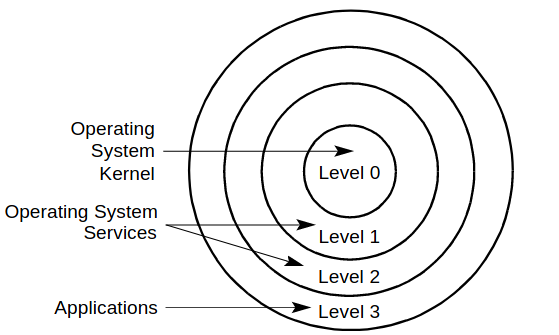
\includegraphics[width=0.5\textwidth]{protection_ring}
    \caption{Protection rings in x86}
    \label{fig:x86}
\end{figure}
In the segmentation approach, memory is divided into multiple segments, with the
most critical ones being the code segment, data segment, and stack segment. Each
segment has its own selector, which is employed to calculate the correct address
by selecting the appropriate segment descriptor from the Global or Local
Descriptor Table (GDT/LDT).The selector can be set by the application while the
descriptor can only be changed by the operating system and is hidden for the
application. These descriptors include a two-bit field known as
Descriptor Privilege Level (DPL), indicating the privilege level that can access
the segment. The CPU stores the Current Privilege Level (CPL) in a register for
segment selectors. Before any other checks, CPL and DPL are compared. If CPL is
equal to or smaller than DPL, access to the memory location is granted, allowing
higher privilege levels to access lower privilege level memory. Otherwise, the
processor generates a general-protection exception. In the event of an
exception, a handler routine is invoked, identified by a segment selector
pointing to a segment descriptor in the GDT or LDT for an executable code
segment. This handler routine may execute at the same privilege level as the
current code segment, as indicated by the DPL of the code segment. If the
privilege levels differ, the stack selector is altered, and CPL is updated to
the new privilege level. This enables the handler to operate at the higher
privilege level.\par
In this context, we can also observe how the concept of modes aligns with
execution semantics. The protection rings embody this semantics by reacting
differently to memory access. In one ring, access is granted, resulting in a
specific state change that we perceive as program execution. In another ring,
the same access or instruction might trigger an exception, leading to a
different state change. The mode switch, as a stateful change of
these semantics, is evident in the update of CPL, which influences the outcome
of the DPL vs. CPL check and consequently the execution of the code. This
underscores the need to reconfigure certain hardware components to establish a
fully software-based mode system. 

\subsection{ARM TrustZone}
TrustZone is a hardware security extension designed for ARM processors \cite{Pinto}. It
serves as an implementation of the Trusted Execution Environment concept. The
primary objective of TrustZone is to partition a processor into two distinct
states: the non-secure mode, which imposes certain restrictions, and the secure
mode, where restrictions are lifted as depicted in Figure \ref{fig:ARM}. This division
operates independently of other ARM modes, meaning that both states support the
usual modes for running an operating system. There are two exceptions to this
rule: the monitor mode, available exclusively in the secure state, and the
hypervisor mode, exclusive to the non-secure state. The monitor mode facilitates
transitions between these two states. In the non-secure state, this mode can
only be accessed through interrupts or the \texttt{SMC} instruction. It is possible to
determine whether an interrupt should trigger a switch to the secure state or be
handled in the IRQ mode within the non-secure state.\par
To implement TrustZone, the entire System-On-Chip (SoC) is divided into these
two distinct states. Isolation can be achieved physically or virtually. For
example, the processor can be time-shared between the two states, giving both
states the illusion of exclusive ownership \cite{ARM}. All hardware components,
including the Level 3 Cache, Memory Controller, DMA controller, and an AXI to
APB Bridge, are interconnected via an AXI bus. This bus incorporates an
active-high non-secure bit (NS). The NS bit is set whenever a memory request has
the Non-Secure Table Identifier (NSTID) bit set, which is the 33rd bit added to
every memory request. It signifies whether the processor is operating in the
secure or non-secure state. Most devices connected to the AXI bus behave
differently based on the NS bit. For instance, the MMU has two virtual MMUs (one
for each mode). The non-secure MMU can only map non-secure memory pages, while
the secure MMU can map all pages. The MMU utilizes a single TLB that employs
tags to differentiate between translations in the two states \cite{ARM}. Caches function
in a similar manner. It's important to note that this is a high-level
description of how these components work, as their operation is highly dependent
on the specific hardware implementation.\par
\begin{figure}[h]
    \centering
    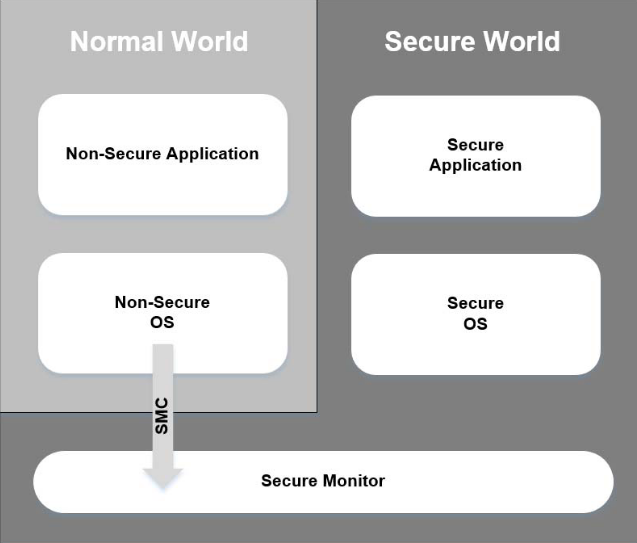
\includegraphics[width=0.7\textwidth]{armtrustzone}
    \caption{TrustZone}
    A division into normal world and secure world is done via hardware on a
    shared processor. Here shown for the ARM Cortex-A architecture.
    \label{fig:ARM}
\end{figure}
This example also illustrates the concept of modes and mode switches. The state
represents a mode and, consequently, an execution semantics. The transition from
one state to another represents a change in these semantics, which can be
interpreted as a mode switch. In this case, the alteration in semantics is more
apparent because it involves a tangible hardware change. In this scenario, the
AXI bus is reconfigured, leading to different interactions with connected
devices or triggering different functions within a device. Trusted Execution
Environments demonstrate the value of adopting a broader definition for modes
and mode switches. With the redesign of software-defined CPU modes, the aim is
to make it feasible to define such environments through software configurations.\par

\section{The RISC-V Architecture}
RISC-V, an open-source Instruction Set Architecture (ISA), has garnered
considerable attention due to its simplicity, versatility, and scalability\cite{Waterman_2}.
Developed at the University of California, Berkeley, RISC-V offers a modular and
extensible framework that caters to a diverse range of computing applications,
from embedded systems to high-performance servers. The choice of RISC-V as the
development platform in this work is motivated by its open-source nature and
relative architectural simplicity compared to x86 or ARM.

\subsection{Privilege Levels}
In traditional processor architectures, CPU modes are typically predefined as
fixed modes, such as kernel mode, user mode, and system mode. However, RISC-V
introduces a more adaptable approach through the concept of privilege levels.
Ranging from M-mode (Machine mode) at the highest privilege to U-mode (User
mode) at the lowest, RISC-V allows for the inclusion of optional S-mode
(Supervisor mode) and H-mode (Hypervisor mode) to address specific use cases.
This flexibility aligns well with the requirements of this work, which deals
with customizability at the hardware level.\par
Privilege levels in RISC-V are realized as distinct hardware extensions, each
bringing its own set of registers and instructions, as described by Waterman et
al.\cite{Waterman}. Moreover, RISC-V can employ various extensions to implement virtual
memory, ensuring memory-level separation. These extensions differ primarily in
the number of page table layers, with this work focusing on the 39-bit virtual
addresses.

\subsection{Privilege Elevation Mechanism}
RISC-V architecture relies on an exception handling mechanism to manage
privilege elevation. Exceptions, deviations from the normal program flow caused
by events like system calls, page faults, or hardware interrupts, trigger
privilege-level switches. \par
To facilitate privilege elevation, RISC-V introduces the "Trap-and-Return"
mechanism. Traps are synchronous exceptions triggered by specific instructions,
such as system calls or illegal instructions. When a trap occurs, the processor
switches to a higher privilege level and invokes a designated trap handler
routine to address the exception. Once the handler completes its task, it
employs the \texttt{mret} (Machine-level return) or \texttt{sret} (Supervisor-level return)
instruction to revert to the original privilege level. For asynchrounous
execeptions such as hardware interrupts the mechanism is the same.\par
Upon exception detection, the processor saves the current program counter (PC)
to the \texttt{mepc} register for machine-mode changes or the \texttt{sepc} register for
supervisor-mode changes. The type of exception is recorded in the \texttt{mcause} or
\texttt{scause} register, and interrupts are disabled by setting the \texttt{sie} bit in the
\texttt{mstatus} or \texttt{sstatus} register. The address of the corresponding trap handler routine is
stored in the \texttt{mtvec} or \texttt{stvec} register, depending on the processor's mode
change. The processor then switches to the target privilege level by
appropriately setting the relevant privilege-level bits in the \texttt{mstatus}
register.\par
During execution of the trap handler routine at the elevated privilege level,
the exception is handled accordingly. Necessary operations, such as servicing
the system call or resolving the page fault, are performed. Upon returning to
the lower privilege level, the processor restores the PC, allowing the program
to continue execution from where the exception occurred. However, tasks such as
saving register state and re-enabling interrupts are the responsibility of the
programmer.\par

\subsection{Memory Protection}
In the context of mode separation, memory protection plays a pivotal
role in ensuring isolation between different privilege levels. RISC-V
employs two distinct memory protection mechanisms: Physical Memory Protection
(PMP) and Paging. \par
PMP serves as a low-level protection mechanism, specifically designed to
safeguard certain regions of physical memory. It grants the Machine mode
exclusive control over configuring PMP settings. However, for the purpose of
this research, PMP's role is relatively minor, and thus, I focus my attention
on the more crucial memory protection mechanism: Paging.\par
Paging serves as the primary defense mechanism for safeguarding kernel memory
against unauthorized access from applications. The Sv39 RISC-V extension enables
this feature. While there are other extensions that support wider
virtual addresses, for the purpose of this thesis, I will concentrate on the
Sv39 extension due to its implementation in gem5 and only minor differences to
other extensions.\par
\begin{figure}[h]
    \centering
    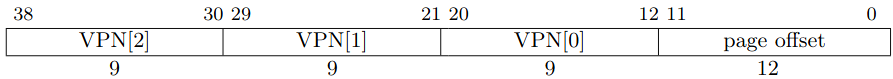
\includegraphics[width=\textwidth]{virtual_ad}
    \caption{Virtual Address}
    A 39-bit virtual address where every VPN[X] entry is an index for the
    corresponing PTE in the page table directory.
    \label{fig:virtad}
\end{figure}
The activation of the paging mechanism involves writing the address of the root
page table into the \texttt{satp} register. In the Sv39 extension, the page table
comprises three hierarchical levels which it's own page directory each. The virtual address undergoes division into
distinct parts (as shown in Figure \ref{fig:virtad}), indicating the index for a
page table entry (PTE) in a page directory. Figure \ref{fig:pte} illustrates a page
table entry with its status bits. The physical address (as shown in Figure
\ref{fig:pad}) is build from the PPN[X] parts of the PTE and the offset from the
virtual address. Any level can contain a leaf. This means Sv39 supports mega and
gigapages. If a such a pages occurs the missing PPN[X] parts in the PTE are
taken from the virtual address like PPN[X] = VPN[X]. Any errors during this
translation process raise a page-fault exception.\par
\begin{figure}[h]
    \centering
    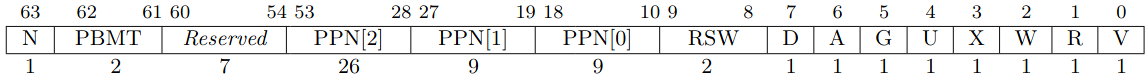
\includegraphics[width=\textwidth]{pte}
    \caption{Page Table Entry}
    A page table entry with various access rights bit at the end. The XWR bit
    indicating read, write and execution rights. If all this bits are zero the
    PTE is pointer to the next level. The V bit indicates if the page
    is valid while U shows if the page is accesible in user mode and G if it is
    a global mapping. Each PTE contains a access (A) and dirty (D) bit.
    \label{fig:pte}
\end{figure}
Each page table contains multiple permission bits, determining access rights to
a memory page. During translation they are checked. If a check fails a
page-fault exception is raised. These permission bits play a crucial role in controlling memory
access and will be expounded upon in detail in the design and implementation
chapter, as they undergo extensive changes throughout the research.\par
\begin{figure}[h]
    \centering
    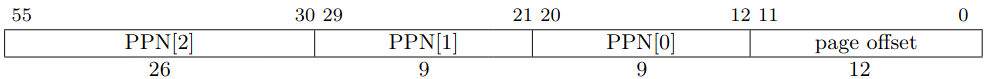
\includegraphics[width=\textwidth]{physical_ad}
    \caption{Physical Address}
    A physical address where the page offset is equal to the offset in the
    virtual address. The PPN[X] either given by the VPN[X] parts of the virtual
    address if it is a mega or gigapage or by the PTE.
    \label{fig:pad}
\end{figure}

\section{The gem5 Simulator}
The gem5 simulator\cite{gem5} stands as a modular full-system simulator,
renowned for its support of diverse instruction-set architectures and hardware
components. Employing a Python interface to interact with hardware components
written in C++, gem5 facilitates the construction of entire systems. This is
achieved by establishing connections between components through ports, enabling
seamless communication via packets exchanged among these interconnected
elements.
The inherent flexibility of gem5 allows for facile modification of packet
handling through alterations in the C++ implementation of objects. This, coupled
with its modular design, expedites the development process, facilitating swift
changes to the Instruction Set Architecture (ISA).
Crucially, for this thesis, gem5 operates on an event-driven model, empowering
precise timing in simulations. Events within gem5 correspond to granular stages,
such as instruction fetch, decode, and execute cycles, facilitating an accurate
simulation down to the timing of individual instructions. This capability to
model specific instructions and actions with precise timings enables a
accurate analysis of design overheads proposed in this thesis

\chapter{Related Work}

This thesis is the continuation of prior work and thoughts on the same and
similar topics. It was motivated by the work of Roitzsch et al.\cite{Roitzsch}
where two different approaches for a new switching mechanism are introduced. One
describing an extra CPU mode acting like a microkernel for mode switch handling
which enables programmable mode switches. The other one raising the idea of a
complete separate CPU which changes the mode of the working CPU and therefore
saving time and memory resources during the switch. The work of von
Elm \cite{Cve} provides a foundation for the creation of such technologies and
will be described in detail in the following chapter.

\section{Programmable Mode-based Memory Isolation}
Von Elm's master thesis \cite{Cve} introduces a RISC-V implementation of
programmable modes, redefining hardware-based mode implementation into a
software-centric paradigm. His approach involves identifying modes through
unique IDs and allocating explicit capabilities based on these identifiers.
Additionally, Von Elm organizes modes in a hierarchical structure, ensuring that
each child mode possesses fewer capabilities than its parent. Notably, this
design has significant implications for mode-specific calling conventions.\par
Calls downward within the mode hierarchy, from parent to child, do not
necessitate special protection, as the parent mode cannot acquire additional
capabilities through this transition. However, calls in the opposite direction
demand heightened security measures. Von Elm implements special semantics for
cross-mode calls, distinguishing between ascending and descending movements in
the hierarchy. For elevations, the call address is not freely selectable,
mandating that each mode possesses a specific entry point for calls originating
from lower hierarchical levels.\par 
The software-based mode implementation proposed by Von Elm raises concerns about
potential performance penalties, primarily if the hardware needs to access
extensive information from memory. To mitigate this, he introduces a cache-like
structure known as the Mode-Lookaside-Buffer. This buffer exclusively resides in
the highest mode, the supervisor mode, and contains vital information about each
mode's attributes, including ModeID, parent mode, entry point, and program
counter (see Fig.\ref{fig:mode_desc}). By centralizing this critical mode
information in the Mode-Lookaside-Buffer, the system optimizes access efficiency
and minimizes performance overhead associated with frequent memory lookups.

\begin{figure}[h]
    \centering
    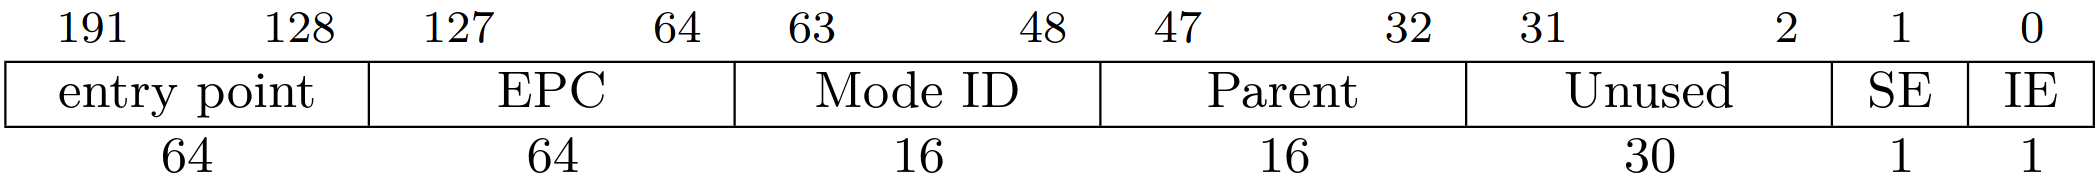
\includegraphics[width=\textwidth]{ue_entry}
    \caption{Mode descriptor}
    \label{fig:mode_desc}
\end{figure}


\subsection{Memory protection for Programmable modes}\label{chap:mem_perm}
A central focus of Von Elm's work involves devising a robust memory protection
mechanism tailored for software-based modes. He adopts a strategy that
split this task into two distinct components. The first task involves
tracking virtual page-to-physical page mappings, while the second task entails
determining access rights allocated to specific memory locations. Von Elm
justifies this partitioning by the potential impracticality of allocating
individual access bits for each mode in the Page Table Entries (PTEs) of a
conventional paging system, as it could lead to unwieldy and oversized PTEs.
However, this approach introduces the challenge of maintaining two separate
systems to accomplish what was previously handled within a single system.
Thus, both systems demand optimal performance for their respective tasks.\par
To address these challenges, Von Elm leverages the efficiency of the regular
paging system for the first task, which minimally impacts the translation
process. For the second task, he implements a segmentation-based approach.
This choice allows us to change permissions more fine-granular. This means it is
possible to use regions smaller than pages and regions that are not
page-aligned. By employing a segmentation model, it becomes possible to
encapsulate the access rights of an entire segment using a single segment
descriptor, rather than employing multiple page table entries (see Fig.\ref{fig:pag_seg}).\par 
\begin{figure}[h]
    \centering
    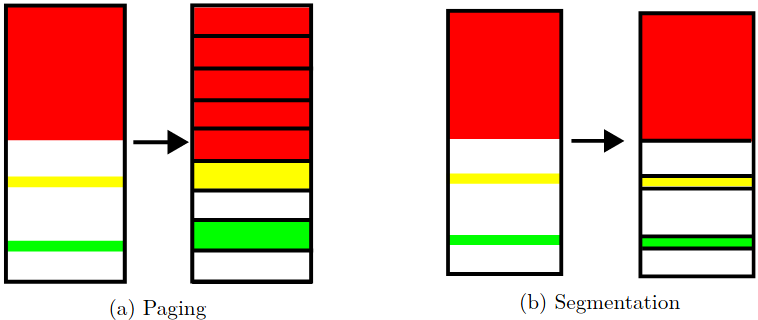
\includegraphics[width=\textwidth]{seg_pag}
    \caption{Paging and Segmentation compared}
    \label{fig:pag_seg}
\end{figure}
For the segmentation-based approach, Von Elm designs a so called
Permission-Lookaside-Buffer (PLB). During the translation phase, this PLB is
consulted to ascertain if a mode possesses permission to access a specific
memory region. Each PLB entry identifies the mode it corresponds to via a ModeID
field and defines the memory region through a start address and an offset,
specifying its size. Access rights are stored using the conventional read,
write, and execute bits, furnishing comprehensive control over memory access
(see Fig.\ref{fig:plb_desc}). This segmented approach offers an efficient means
of managing memory protection, striking a balance between performance and
granularity in access control for software-based modes.
\begin{figure}[h]
    \centering
    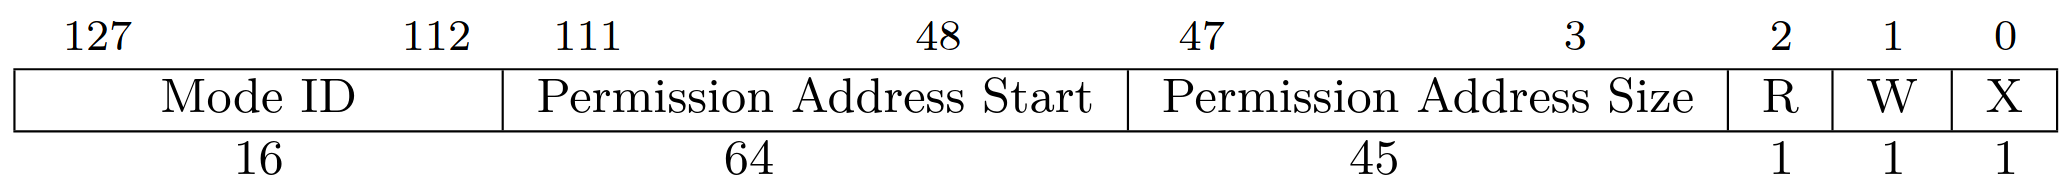
\includegraphics[width=\textwidth]{ue_plb}
    \caption{PLB descriptor}
    \label{fig:plb_desc}
\end{figure}
\chapter{Design}
In this chapter, I aim to present two distinct designs for implementing
software-defined CPU modes. The primary approach under discussion involves the
integration of a single hardware supported CPU mode  that enables the definition
of additional modes in software. The difference to "Programmable Mode-based
Memory Isolation" is a more flexible approach. There is no more hierarchy between
modes and no hardware defined mode switch behavior. I will delve into the
specific hardware components that necessitate migration to software to support
this concept. Additionally, I will expound upon the methodology for defining and
storing modes while identifying the requisite new instructions to be
incorporated into the Instruction Set Architecture (ISA).\par
The second design I will explore introduces an additional core to our CPU,
selectively activated for mode switching, accounting, and CPU reconfiguration
purposes. This innovative design anticipates addressing potential performance
bottlenecks that may arise from executing mode handling on the same core. I will
explain which CPU components must be made accessible by this supplementary
core to ensure seamless functionality. Moreover, I will examine the feasibility
of incorporating elements from the extra mode design onto the supplementary CPU.  

\section{Mode Switch Mode}
This section will present the design of an additional mode, termed as the "Mode
Switch Mode," dedicated to managing mode switching and definitions within the
CPU architecture. The Mode Switch Mode serves as the sole mode defined by the
hardware, equipped with the capability to define other modes. It operates as a
programmable supervisor mode for mode creation and seamless transitions between
them, allowing software to freely define the target mode and actions during the
transition. This programmability enables dynamic mode management, entirely
controlled by software interventions.\par
To enable this functionality, specific alterations to the CPU architecture are
necessary. In Figure \ref{fig:msm_schema} you can see that there are two new
control and status registers added in. The interrupt and fault handling
mechanism where restructured and some new structures, the Mode-Lookaside-Buffer
and the Permission-Lookaside-Buffer where added to the MMU. To use some of this
changes new instruction have been added and the preexisting \texttt{mret} has
been altered. In the subsequent sections I will explain this changes in more detail.

\begin{figure}[h]
    \centering
    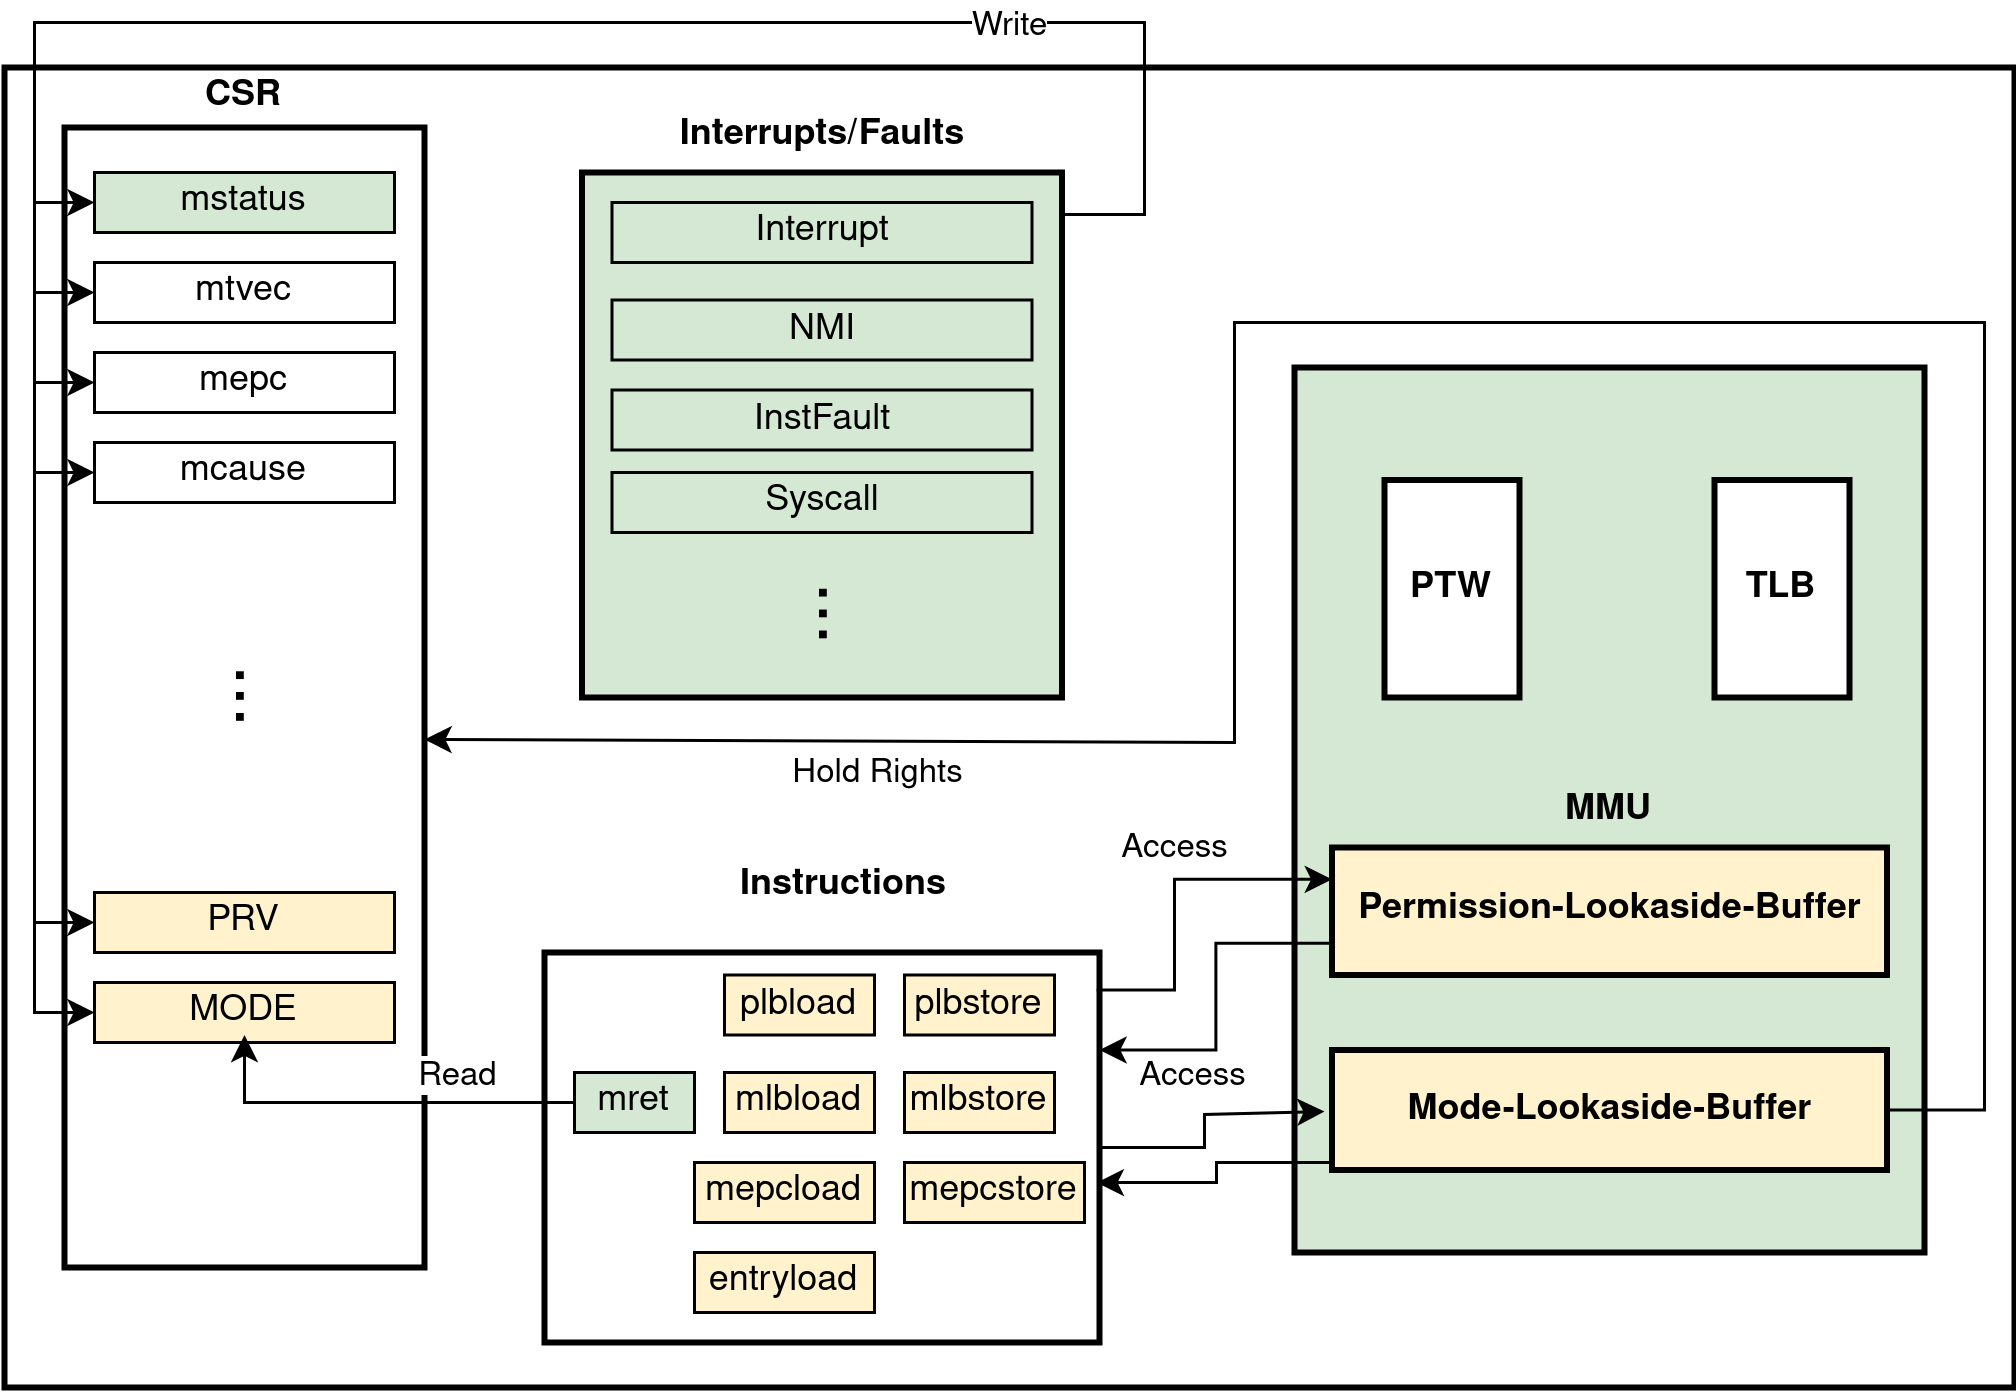
\includegraphics[width=1\textwidth]{MSM_schema}
    \captionsetup{justification=centering}
    \caption{Schema for the Mode Switch Mode}
            Yellow symbolizes elements that are newly added, green marks
            elements which were in the original Risc-V design and have now a
            slightly different design. 
    \label{fig:msm_schema}
\end{figure}

\subsection{Modes}
The first question to answer was how modes are defined. Should modes be
implicitly identified by the resources which are currently available or should
they be explicitly identified by an Id ? I decided to implement modes explicitly
because it seems easier to create a flexible design where modes can be created
and accounted during runtime with Ids instead of always keeping track which
resources are made available at the current time.\par
Another question is should this modes have a hierarchy or be completely free
standing. One could argue that a hierarchical approach makes sense to keep track
of which mode can destroy or create an other mode. Further it eases some
security checks regarding child calls, so that a mode can not call arbitrary
into an other mode as Von Elm describes it in his thesis. Figure \ref{fig:free_schema} shows what would
need to be done to change from a one mode to another with in a hierarchy. The
call to the parent would be implemented in hardware and therefore add some
implicit security. In a freestanding design such a jump to the parent also
happens. In this case the Mode Switch Mode can be seen as the parent mode where
arbitrary calls are not possible. So a free standing implementation of the
modes wouldn't change much of the behavior but adds more flexibility for the
Mode Switch Mode. Therefore I decided to use a free standing implementation of
modes.

\begin{figure}[h]
    \centering
    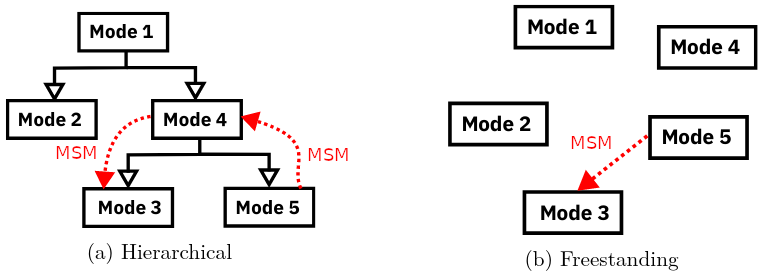
\includegraphics[width=1\textwidth]{free_vs_hier} 
    \captionsetup{justification=centering}
    \caption{Hierarchical and Free-standing mode switch}
            The red arrow denotes what it takes to change the mode. Every MSM
            shows when the Mode Switch Mode is entered. The Mode Switch Mode
            acts as a parent mode in the freestanding implementation where an
            arbitrary jump is not possible. It just enables a more flexible
            design of how to switch modes. A hierarchy where a jump is routed
            through a parent mode just increases the number of modes that are
            entered.
    \label{fig:free_schema}
\end{figure}

\subsection{Mode Accounting}
Following the introduction of modes, I want to show how modes are accounted in
efficient way. This is crucial because the mode restoration could otherwise impose a
significant overhead on the Mode Switch which should be as quick as possible.
Addressing this issue, Von Elm\cite{Cve} encountered a similar challenge and
devised a solution in his work. He proposed a Mode-Lookaside-Buffer(MLB)
architecture to store mode descriptor which hold all necessary information
about a modes state and access rights.\par
I decided to use the same infrastructure for this project. For this work I
created the following mode descriptor(see Fig.\ref{fig:mode_descriptor}) along
some special instructions for altering it which are only available in the Mode
Switch Mode. The first 64 bit of the mode
descriptor are for a entry point into the mode. This can be used to access a
mode if it has never been run before and has no current program counter or if
this mode has a handler routine which should be called on entering this mode. To
load the address from this field the \texttt{loadentry} instruction was created
to quickly load this address. There is no special write instruction to this
field, because once it is set it shouldn't be changed anymore. Because of this
the entry point field should be set on creation of a mode descriptor when it is
saved with the \texttt{mlbstore} instruction. The whole descriptor can be loaded
for later alteration with the \texttt{mlbload} instruction but this is a
performance heavy access because we now have one load and one store instruction.\par
The second 64 bit hold the program counter. This field can be used if a mode
should restart its execution at a certain point for example when it is
interrupted or made a system call after which it wants to reenter its own
control flow. Because this field can be written on every mode switch, there is
the \texttt{mepcstore} instruction which writes an address to the \texttt{EPC}
field of the mode descriptor. It can be restored with \texttt{mepcload}. The
handling which address should be loaded, either the entry point or the last
program counter, can be implemented in the mode switch mode by the systems
programmer.\par
The next 16 bit of the descriptor are the Id which is used to identify modes.
Because it should only be set on mode creation there are no special instructions
to read or write this field. It is mostly used in hardware to find check if a
mode has certain rights and to find a mode if a \texttt{mepcload} or an other of
the special instructions is used.\par
The next 3 bits are currently unused but could implement some interrupt
forwarding capability in the future. The last 45 bits are used to describe
access rights to the control and status registers. Due to its complexity this
topic will be discussed in the next section.

\begin{figure}[h]
    \centering
    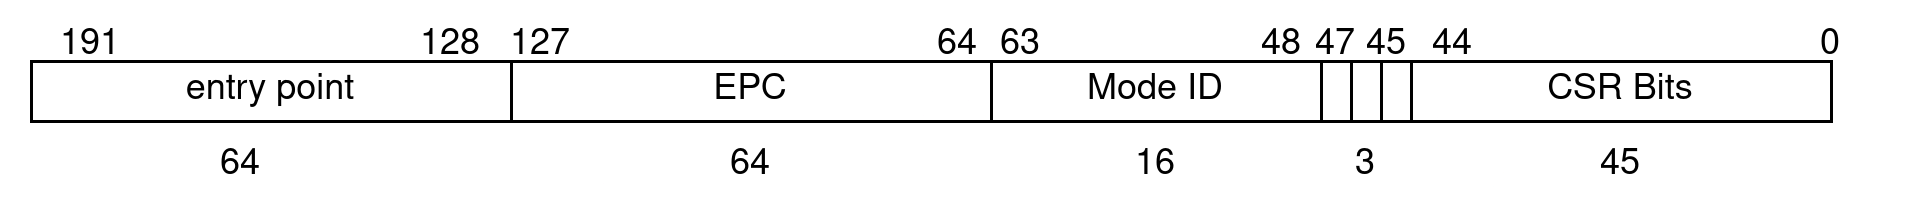
\includegraphics[width=\textwidth]{modeentry}
    \caption{Mode descriptor}
    \label{fig:mode_descriptor}
\end{figure}

\subsection{Control and Status Registers}
One of the core parts of mode isolation in RiscV are the control and status
registers. Some of them are only accessible in a certain mode. To give the full
control about mode creation this rights need to be dynamically changeable. This
is done with the last 45 bits of the mode descriptor. The bits represents the
access rights to the CSRs. If this bit is set a mode has read and write access
to this CSR. To reduce the amount of bits for all 119 CSRs some of them are
grouped together. This means from bit 44 till bit 2 they represent all CSRs from
top to bottom without the HPM und PMP registers because if a mode have access to
one of the HPM or PMP registers, it should have access to all of the HPM or PMP
registers. This means that bit 1 represents access to the HPM registers and bit
0 represents access to the PMP registers. In RiscV the CSRs are written with
special \texttt{csrr} instruction. On execute of this instructions a check is
run against the mode descriptor if this instruction is possible.\par
This check uses the \texttt{prv} CSR which holds the current mode to identify
against which descriptor should be checked. The access rights of \texttt{prv}
can not be changed and it is only writeable by the hardware. This
CSR was newly introduced to hold the mode id of the currently running mode.
As you can see in Figure \ref{fig:msm_schema} another new CSR is the \texttt{mode} field which
holds the previous mode while the Mode Switch Mode is entered and holds the
target mode when the Mode Switch Mode is left.\par
The only way to change the \texttt{prv} CSR is the \texttt{mret} instruction. It
is only available to the Mode Switch Mode and is used to change back from the
Mode Switch Mode to any target mode. Therefore the \texttt{prv} register is set
to the value of the \texttt{mode} register effectively changing the mode of the
CPU. During the \texttt{mret} the interrupt enable bit in the \texttt{mstatus}
is not changed enable the programmer to allow mode switch with disabled
interrupt for example when entering an interrupt handler in a special interrupt
handling mode. The program counter for the entered mode is loaded from the
\texttt{mepc} register.

\subsection{Traps and Mode Change}
After detailing the methods to access and manipulate different CPU states and
modes, I want to explain how the transition into the Mode Switch Mode
occurs and which information is preserved during this process.\par
Every trap, encompassing interrupts, faults, or syscalls, redirects control flow
into the Mode Switch Mode. During this transition, interrupts are disabled,
ensuring entry into the Mode Switch Mode with interrupts turned off. The current
program counter is preserved within the \texttt{mepc} register, while the program counter
is set to the value contained in the \texttt{mtvec} register. The mode which we
are leaving is written to the \texttt{mode} register. All other registers treated like in
an normal RiscV implementation.\par
\vspace{12pt}
Having explained the essential building blocks necessary for a
simple transition from the Mode Switch Mode to another mode, I'll provide a
quick overview of how the mode descriptor and the new CSRs work together.\par
Upon arrival at the Mode Switch Mode, the program counter for the previous mode
is loaded from the \texttt{mepc} register and then stored via the
\texttt{mepcstore} instruction into the mode descriptor. The mode Id for this
descriptor can be retrieved from the \texttt{mode} register. Subsequently, the Mode Switch Mode determines
the correct mode to switch to. Once this mode is identified, the address where
the new mode starts can be loaded, either with \texttt{mepcload} or
\texttt{entryload} from the according mode descriptor field. The loaded address
is then stored into the \texttt{mepc} register.\par 
Concurrently, the \texttt{mode} register is updated with the ID of this newly
targeted mode. If the new mode is intended to start with interrupts enabled,
this setting should be enabled at this stage by the Mode Switch Mode code.
Finally, invoking the \texttt{mret} instruction effectuates the mode change.
These outlined steps constitute the minimal procedural actions when
transitioning from one mode to another. However, additional steps, such as
saving specific registers  can also be incorporated.\par
Regarding the initial configuration, upon processor boot-up, the system
starts in the Mode Switch Mode, allowing for essential configurations. The
\texttt{mtvec} register should be set to point to the handler of the Mode Switch Mode.

\subsection{Memory Protection}
An essential aspect of modes is memory protection, particularly in the context
of memory virtualization. As the number of modes increases, the traditional
paging approach faces limitations. The conventional paging system encounters
challenges in efficiently storing access information for each mode within the
page table entry, especially with a rapidly escalating number of permission bit entries even
for a relatively small number of modes. A proposed solution is to split the
accounting and permission handling parts, typically executed simultaneously.
This separation is due to the inherent strength of paging in accounting for
memory locations with uniform sizes but lacks efficiency in verifying access
rights for irregularly shaped memory segments composed of multiple pages (for
further insights, refer to Chapter \ref{chap:mem_perm}).\par
Addressing this challenge, Von Elm et al.\cite{Cve} have already provided a solution. He
leverage the paging method for accounting purposes, as the page table walk
offers the most compact footprint to record the relationship between physical
and virtual memory. For the access rights control aspect, they employ a
segmentation-based approach. Here, memory locations starting from a designated
start address and ending at an address calculated by an offset from the start
address possess certain access rights. The page-permission bits will remain
as-is. The permissions assigned to a memory address in this setup represent the
minimum of the permissions granted by both the paging and mode systems. In cases
where the mode system designates read and write permissions for an address,
while the page table specifies read and execute permissions, the address will
only be accessible for reading. To define these memory locations, a segment
descriptor (illustrated in Fig. \ref{fig:plb_descriptor}) is formulated,
encompassing details such as the start address, offset, and permission bits.\par

\begin{figure}[h]
    \centering
    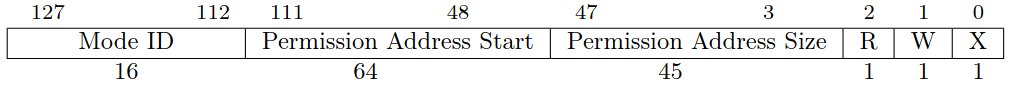
\includegraphics[width=\textwidth]{plb}
    \caption{PLB descriptor}
    \label{fig:plb_descriptor}
\end{figure}

To optimize performance, this descriptor is loaded into the
Permission-Lookaside-Buffer (PLB), allowing the Memory Management Unit (MMU) to
efficiently fetch information regarding access rights during the page table
walk. Programmers can populate this buffer using the \texttt{plbstore} and \texttt{plbload}
instructions within the Mode Switch Mode. The segmentation layer always needs to be
configured on top of the paging layer. Given that the primary focus of this
work isn't solely on memory protection, I integrated this working
solution into my design to address this crucial aspect.

\section{Control Core}
This section explains the second approach involving an additional core
dedicated to managing all mode switch activities. Named the Control Core, this
entity exists alongside the CPU as an independent unit with its dedicated
memory(see Fig. \ref{fig:cc_schema}). Conceptually, it resembles an accelerator
where the CPU delegates all mode switch responsibilities. The Control Core
encompasses all functionalities offered by the Mode Switch Mode.\par
The rationale behind this approach lies in the anticipation of performance
benefits by offloading mode switch handling onto a secondary core equipped with
its own registers. If the Mode Switch Mode runs on the same CPU whenever a this
mode is entered and want to use some registers, the used registers need to be
saved and restored before we are leaving this mode. As the Mode Switch Mode is
basically just an abstraction of a quick state change that was done in hardware
before it should have the least overhead possible to not bottleneck the
performance of the CPU. On a secondary CPU this saving and restoring of
registers is not necessary anymore. Now the only overhead is the one of
activating the new CPU. The impact of this will be discussed in the evaluation
chapter.\par 
In Figure \ref{fig:cc_schema}, the overall structure of this approach mirrors that
of the Mode Switch Mode. Similar strategies are adopted for storing modes and implementing
memory protection. However, a notable distinction lies in the distribution of
buffers. The Mode-Lookaside-Buffer is connected to both CPUs to ensure a rapid
access by the control core to handle modes and checks for access rights to the
control and status registers by the main CPU. The Permission-Lookaside-Buffer is
exclusive to the real CPU because memory protection occurs solely within the real CPU,
as different modes operate within this domain, while the memory allocated to the
Control Core can be seen as a scratchpad memory. This memory is exclusively used
by the control core and does not need any address translation or protection.\par

\begin{figure}[H]
    \centering
    \includegraphics[width=1\textwidth]{CC_schema}
    \caption{Schema for the Control Core}
    \label{fig:cc_schema}
\end{figure}

The principal divergence is evident in the Control Core having its dedicated
memory and registers. This distinction becomes particularly salient during the
transition from a mode to the Control Core in the event of a trap. Additionally,
questions regarding the extent of access the Control Core should possess over
the real CPU and the requisite new instructions to facilitate this access will
be examined in subsequent sections.

\subsection{Control Core access}
In addressing the question of accessing specific states on another CPU,
we first have to answer the question which states needs to be read and
changed to fulfill a mode switch. After discussing this question of what must be
changed, I will answer how this changes are done\par
Primarily, the control and status registers stand out as imperative entities
necessitating read and write operations. Initially, retrieving the CPU's current
state requires reading from these registers, while altering the state of the CPU demands
subsequent write operations to the CSRs. Access to this registers is still
handled via the bits in the mode descriptor which is write and readable form the
Control Core with the \texttt{mlbstore}, \texttt{mlbload}, \texttt{mepcstore},
\texttt{mepcload} and \texttt{entryload} instructions. The decode unit of the
main CPU can also read this entries to make the necessary checks on access
rights. Therefore the MLB is connected to both the main CPU and the Control
Core, as you can see in Figure \ref{fig:cc_schema}.\par
Another crucial aspect requiring read and write access is the
Permission-Lookaside-Buffer (PLB). Despite the Control Core not mandating memory
protection, it initiates the creation and modification of entries in the buffer.
However, the general-purpose registers, while essential for facilitating communication
between CPU modes and the Control Core (e.g., syscalls specifying mode creation
or transitioning to another mode), do not essentially require write access from
the Control Core. Changes within these registers should occur exclusively within
modes to make the mode switch transparent to the modes. Although in future scenarios it
could be useful the change certain registers.\par
Having identified the CPU components requiring accessibility, a suite of
instructions to accomplish these tasks is introduced. For accessing the CSRs,
the \texttt{f_scsr} (foreign store CSR) and \texttt{flcsr} (foreign load CSR)
instructions are devised to store to and load values from the CPU's CSRs, either
to or from the Control Core's registers.\par
To alter access bits and modify PLB entries, instructions such as
\texttt{plbstore} and \texttt{plbload} from the Mode Switch Mode are employed
with alterations for this specific scenario. All the introduced instructions,
executed on the Control Core, effectively alter the CPU's state.\par
Regarding regular registers, although not essential, an instruction is included
to read and write them, despite the absence of a current use case. The
\texttt{rfr} (read foreign register) instruction reads a register from the CPU
designated by its index into a target register within the Control Core.
Conversely, the \texttt{wfr} (write foreign register) instruction writes a value
from a register on the Control Core to another identified by its index on the
CPU.


\subsection{Traps and Core Change}
Having explained how the Control Core interacts with the CPU, it's pivotal to
describe the activation process of the Core. This process bears resemblance to a
transition into the Mode Switch Mode. Consequently, the CPU's mode is preserved
in the \texttt{mode} register, accessible for reading by the Control Core.
Simultaneously, the current program counter of the CPU is stored in the
\texttt{mepc} register. The Control Core's program counter is then initialized
to the standardized start address, 0x82000000. This uniform starting address
ensures the Control Core consistently operates as a handler, facilitating
seamless initiation at a predefined location. Subsequently, the CPU is halted,
and the Control Core is initiated. As observed in the Mode Switch Mode, all
other registers are managed similarly to a standard RISC-V CPU during this
process.\par
Returning from the Control Core is facilitated by the \texttt{mret} instruction.
The CPU's \texttt{prv} register is populated with the mode ID retrieved from the
\texttt{mode} register, while the program counter is loaded from the
\texttt{mepc} register. Consequently, the Control Core is halted, and the CPU is
reactivated. Notably, the interrupt bit in the \texttt{mstatus} register remains
unaltered during the transitions. The decision to activate interrupts upon mode
initiation or not resides entirely with the Control Core, ensuring flexibility
in managing interrupt enablement at the mode level. 

\chapter{Implementation}
This chapter is dedicated to presenting a prototype implementation of the
previously discussed designs within the gem5 simulator. The main goal here is to
provide a comprehensive overview of critical implementation details, showcasing
how these designs are brought to life within the gem5 environment. It will also
highlight the addition of new instructions to the compiler, which are used by
the software that runs on the gem5 simulator. 

\section{Mode Switch Mode}

\begin{figure}[h]
    \centering
    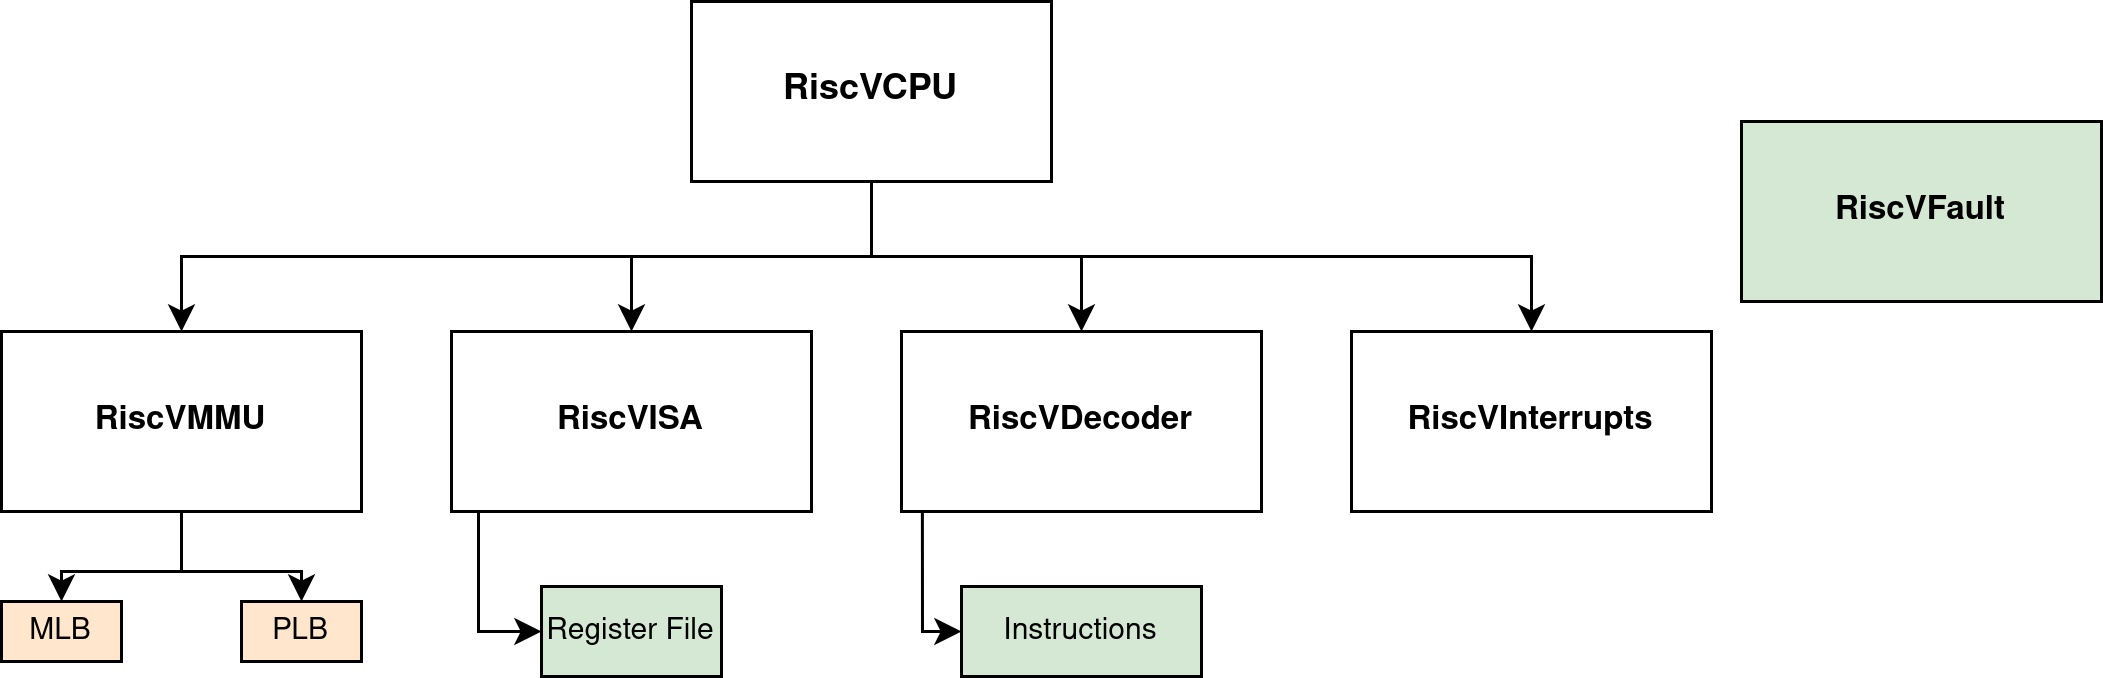
\includegraphics[width=1\textwidth]{overview_im}
    \captionsetup{justification=centering}
    \caption{Overview over the gem5 Risc-V building blocks}
            Yellow symbolizes elements that are newly added, green marks
            elements which were in the original Risc-V implementation and have
            now a slightly different one. 
    \label{fig:overview_im}
\end{figure}

The gem5 simulator has already implemented Risc-V as a usable processor type.
This processors internal structure comprises multiple interconnected C++ classes
and is utilized within simulations as a Python Class. When employing
this processor in a simulation, it instantiates a Risc-V CPU, serving as the
primary implementation of the Risc-V architecture within gem5. This CPU
comprises four primary modules: the Risc-V MMU, Risc-V ISA, Risc-V Decoder, and
Risc-V Interrupts (refer to Fig.\ref{fig:overview_im}). The RISC-V MMU managed
memory requests and acting as an interface between CPU, memory and caches.
The Risc-V ISA module manages the CPU's state, including control over the
program counter, outstanding faults, and crucially, the CPU registers. It
provides an interface to interact with these registers, considering the
potential side effects of such interactions, including checks against privilege
levels. Consequently, any register implementation occurs within this module. The
Risc-V Decoder interprets the incoming binary instruction stream, employing
auto-generated execution modules to execute individual instructions. The
instructions are defined in a specialized ISA description language,
which is the most important aspect of implementing new instructions.
Another crucial component is the Risc-V Fault module, encompassing events triggered by
the simulation to manage the changes that any kind of fault induces
within the CPU. This module is essential for facilitating transitions into the
Mode Switch Mode. The Risc-V Interrupts module primarily checks for interrupt occurrences and
triggers a fault event if such a check confirms an interrupt. Additionally, it
sets a bitmask within certain control and status registers. While minor
adjustments are made to the bitmask, the majority of this module remains
unchanged for this specific work.\par
I adopted the solution proposed by Von Elm et al.\cite{Cve} for both MLB and PLB,
seamlessly integrating it into the MMU of the RISC-V CPU. This implementation
was employed to access Memory Lookaside Buffers (MLB) and Permission Lookaside
Buffers (PLB) while handling instructions. In each pagetable walk conducted by
the pagetable walker integrated into the MMU, the PLB is utilized to verify
segmentation rights. The inclusion of the MLB in the MMU is justified by its
role as a cache for modes, making it appropriate for implementation within the
module responsible for managing these aspects. To align with the specifications
outlined in the design chapter, I introduced minor modifications to the entries
for encoding relevant information. Additionally, within the MLB, I introduced a
method \texttt{can\char`_access\char`_csr} which takes a mode ID and a CSR number as inputs,
verifying whether the mode possesses the necessary access rights to the CSR.
This method emulates a hardware check performed by the MLB.\par
Within the Risc-V ISA module, I removed all references and checks related to
modes. I augmented the \texttt{vector} that defines the CSRs
by introducing new fields representing the \texttt{prv} and
\texttt{mode} registers. Upon initialization, the current mode is set to the
Mode Switch Mode instead of machine mode.\par
In the Risc-V Decoder, specifically in the ISA description, I modified all existing
functions that read or write a CSR to validate if such operations are
allowed in the current mode. This validation is achieved by calling
\texttt{can\char`_access\char`_csr} from the MLB with the current mode and the
CSR intended for access. Furthermore, I included the new instructions introduced
in the design chapter.\par
Significant modifications were made in the Risc-V Fault module. All alterations
specific to modes in certain registers or the CPU state were removed. Instead
the Mode Switch Mode is entered without any changes to the current registers. To
do this the program counter, which is reset here, is set to the entry point of
the Mode Switch Mode. The mode which is left is saved to the \texttt{mode} field
in the CSR vector while the \texttt{prv} field is set to 1 which represents the
Mode Switch Mode. These module changes apply solely to the full system
simulation, as only this simulation replicates CPU changes.\par 

\section{Control Core}
For the Control CPU, I opted to employ two Risc-V processors, both implementing
the Mode Switch Mode. Certain alterations were made to the ISA, which I will
elaborate on later. Firstly, I aim to clarify the overall structure necessary to
realize this design.\par 
As depicted in Figure \ref{fig:python_im}, I interconnected two Risc-V CPUs
through a crossbar, establishing a link to the main memory. Alongside these two
CPUs, there exists two PIO devices connected to the same crossbar. One of the CPUs is
designated as the main CPU, while the other serves as the Control Core. The PIO
devices, which respond to writes at specific addresses, function as handlers for
both CPUs. In the event of a trap occurring at the main CPU, the RiscVFault
module is configured to issue a write to the \emph{main CPU} PIO device's address, activating
it. Subsequently, this PIO device deactivates the main CPU and sets the program
counter of the Control Core to a fixed handler address. The Control Core's
wake-up is scheduled using a gem5 event. Activating the Control Core through a
gem5 event offers the advantage of introducing a customizable delay. The return
path from the Control Core to the main CPU follows a similar procedure. Once the
Control Core completes its execution, it returns to the main CPU using the \texttt{mret}
instruction. This instruction triggers a write to the \emph{cc} PIO device's address
causing the PIO device to deactivate the Control Core and activate
the main CPU through another gem5 event. The main CPU then resumes execution in
its current state, configured appropriately by the code on the Control Core.
The decision to implement two fully developed CPUs was driven by the ability to
write code for the Control Core in standard RiscV assembly and leverage the
existing toolchain for building on it. This system configuration was established
using the gem5 python build tools.\par

\begin{figure}[h]
    \centering
    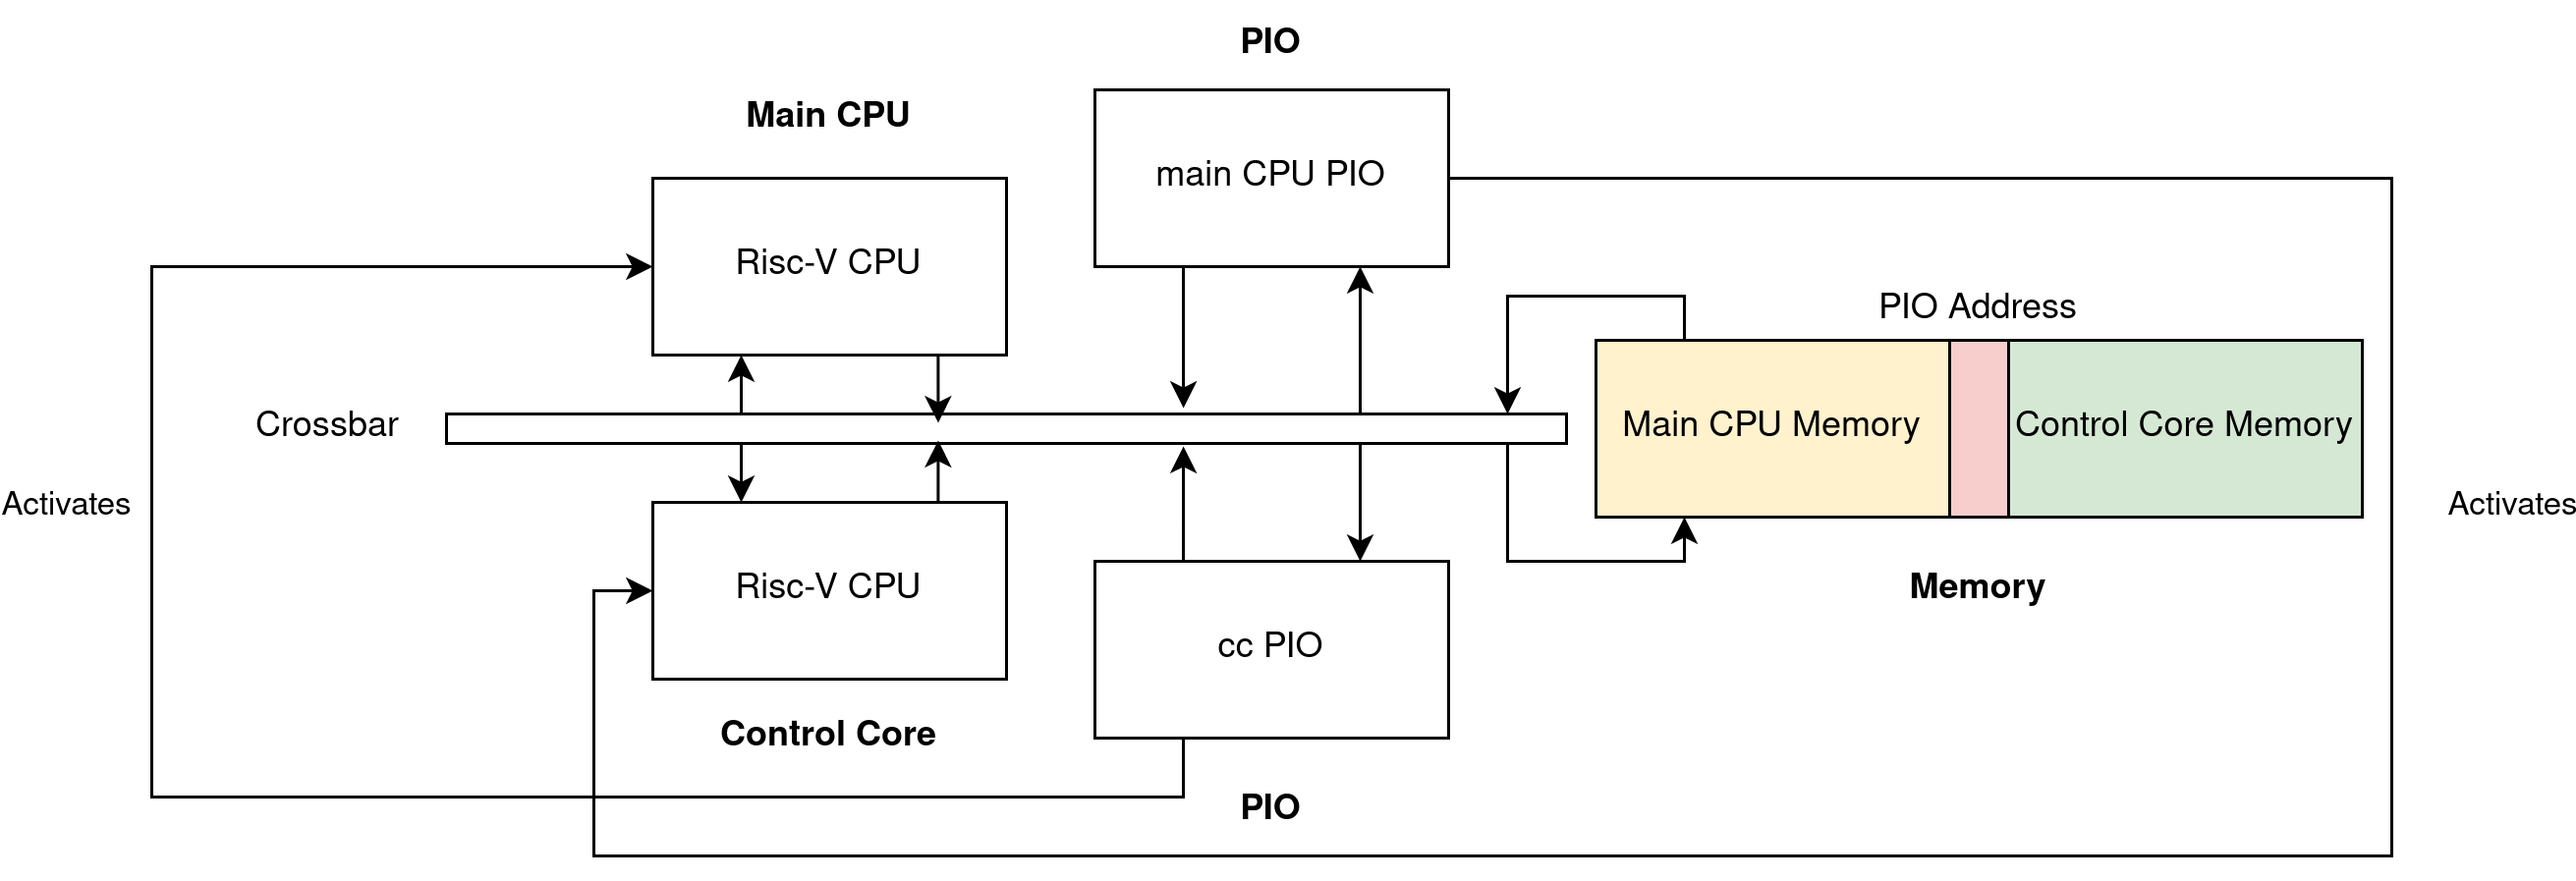
\includegraphics[width=1\textwidth]{python_im}
    \captionsetup{justification=centering}
    \caption{Schema of the Control Core}
        Two dedicated memories for each subsystem for memory isolation. The PIO
        device activates the CPUs of the different systems.
    \label{fig:python_im}
\end{figure}

Within the Risc-V ISA module, a new pointer named \texttt{foreign\char`_isa} is introduced.
This pointer stores a reference to the Risc-V ISA module of another CPU. During
simulation setup, this pointer is initialized with a reference to the Risc-V ISA
module of the other of the two CPUs. This allows access to the registers of the other CPU
through special instructions described in the design chapter. These instructions are
implemented within the ISA description of the Risc-V Decoder. Ordinarily, a
register-altering instruction invokes one of the register access functions of
the current ISA. However, an instruction accessing the registers of the other
CPU uses the \texttt{foreign\char`_isa} to invoke the same functions on the other
CPU. Instructions utilizing this pointer are limited to the Control Core, and if
employed on the main CPU, they result in an illegal instruction fault.

\section{Compiler Instructions}
To facilitate the utilization of the newly introduced instructions, I opted to
integrate them into the GNU assembler. This integration requires four key
components: the instruction's name, format, mask, and match. The RISC-V project
provides the riscv-opcodes tool, enabling the derivation of the mask and match
for an instruction from its string representation. Once obtained, along with the
instruction's name and format, these components can be seamlessly implemented
directly into the GNU assembler. This integration enhances the ease of use for
developers leveraging the modified instruction set within the GNU assembler
environment.
\chapter{Evaluation}
In this chapter, I provide a overview of the methods and tests
conducted in the context of my research. The primary focus involves a
comparative analysis of the two introduced designs through various
microbenchmarks. The overarching objective is not solely to contrast these two
designs but to establish a threshold for the activation time of the Control
Core. Additionally, I aim to determine the point at which a transition to a
different core becomes beneficial in terms of the quantity of saved registers
that do not require preservation on the Control Core.

\section{Benchmarks}
For the benchmarks employed in this study, I devised two distinct
scenarios to facilitate the testing process. The first benchmark involves a
straightforward system call-like entry into the Mode Switch Mode, followed by a
return to the original mode. In this case, since there is no transition to
another mode, only three temporary registers are preserved to provide the Mode
Switch Mode with some registers to utilize. It's worth noting that on the
Control Core, such preservation is unnecessary due to its inherent structure,
which includes dedicated registers for its operations. The primary objective of
this particular test is to identify a threshold at which the transition to a
second CPU becomes too expensive. Therefore this benchmark is run with a variety
of delay timings for Control Core activation. To simulate both directions
of the activation process, this delay is incorporated during the activation of
both the Control Core and the main CPU. It is given in the time that one
instruction takes to be executed. So a delay of one means that the activation of
the other core takes the time that one instruction would take to execute. The
general control flow of this benchmark is illustrated in Figure
\ref{fig:syscall}.\par

\begin{figure}[h]
    \centering
    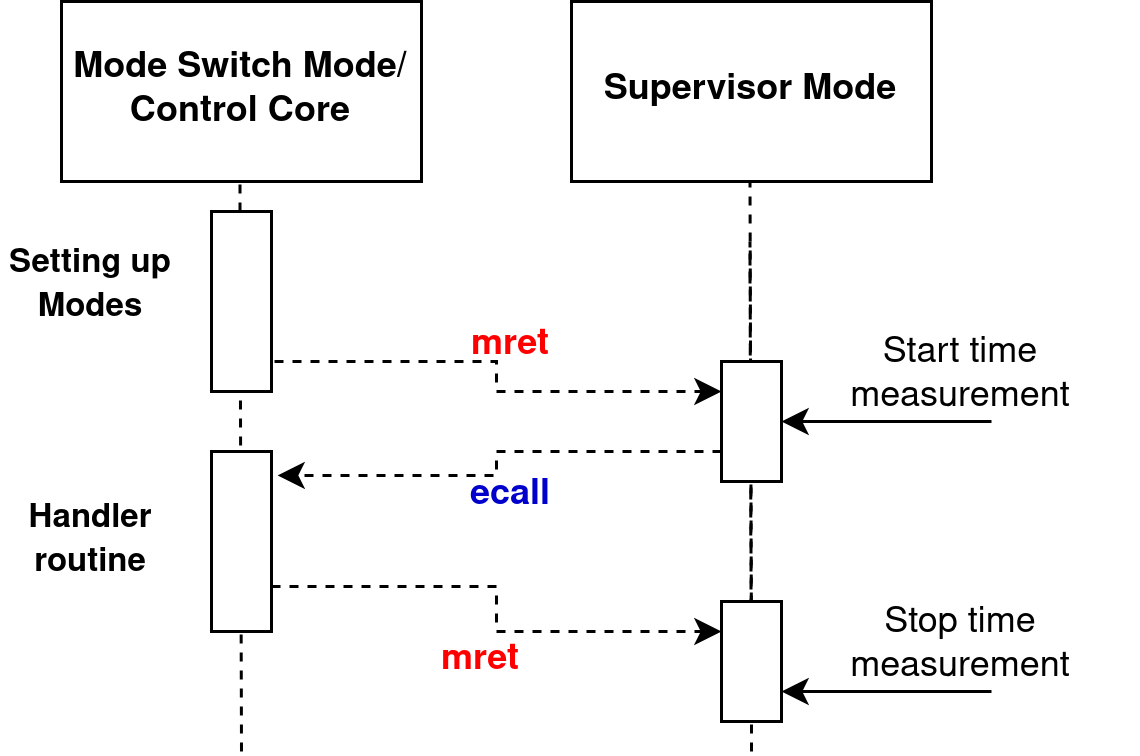
\includegraphics[width=0.5\textwidth]{syscall}
    \captionsetup{justification=centering}
    \caption{Control Flow for simple call into the Mode Switch Mode}
            The control flow changes that happen during a call from the
            supervisor mode (the start mode) into the Mode Switch Mode and back.
            Red depicts instruction executed by the Mode Switch Mode or Control
            Core, blue instruction executed by the other modes. The start and
            end of the timing measurements before and after the \texttt{ecall}
            in the supervisor mode is marked. 
    \label{fig:syscall}
\end{figure}

The second benchmark emulates a comprehensive mode switch from one mode to
another. As depicted in Figure \ref{fig:modeswitch}, the original mode is exited, and the Mode
Switch Mode or Control Core assumes control of the mode-switching process.
Subsequently, the new mode is entered, quickly transitioning back into the Mode
Switch Mode or Control Core, which then transfers control back to the initial
mode. The objective of this benchmark is to identify a threshold of
registers that should be preserved, determining the point at which it becomes
advantageous to switch to a different CPU that doesn't necessitate such
preservation. To ascertain this threshold, the benchmark is executed with
varying numbers of saved registers.\par

\begin{figure}[h]
    \centering
    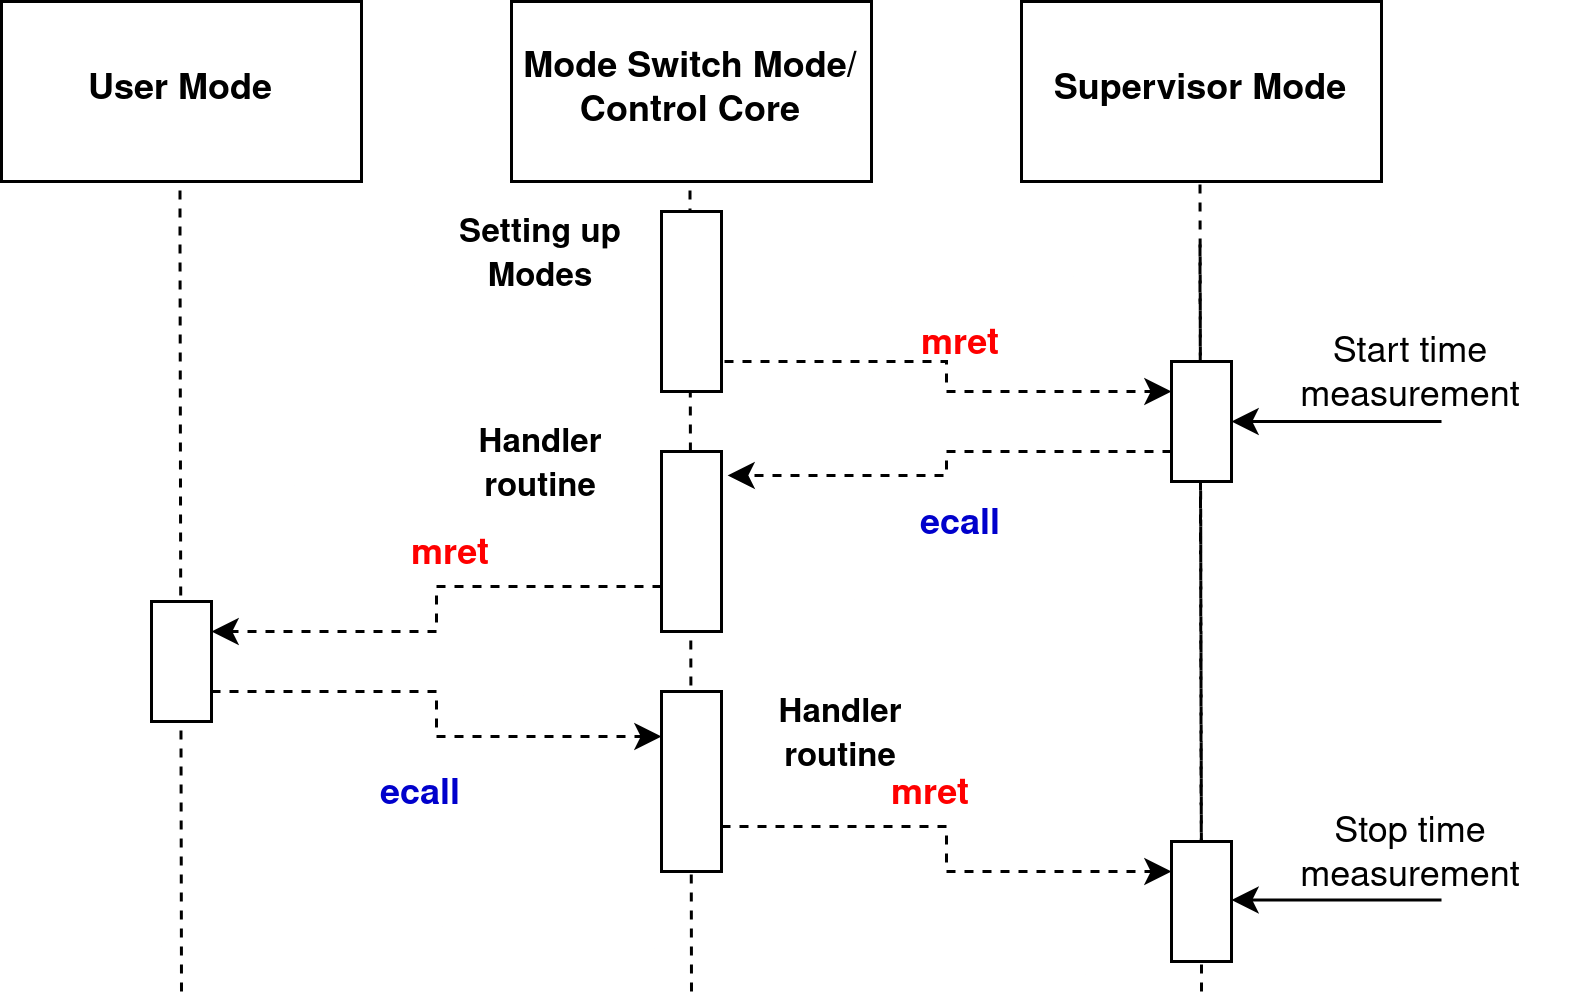
\includegraphics[width=0.8\textwidth]{modeswitch}
    \captionsetup{justification=centering}
    \caption{Control Flow for a mode switch}
            The control flow changes that happen during a transition from the
            supervisor mode (the start mode) to the user mode. Red depicts
            instructions executed by the Mode Switch Mode or Control Core, blue
            instructions executed by the other modes. The start and end of the
            timing measurements before and after the \texttt{ecall} in the supervisor
            mode is marked. 
    \label{fig:modeswitch}
\end{figure}

In both scenarios, the mode switch is initiated through the \texttt{ecall}
instruction from the mode which is left. Therefore the mode switch can be seen
as a ``system call" to the Mode Switch Mode
or Control Core with a request to transition to a specific mode. Notably, this
system call does not include any arguments, as the current routine for mode
switching is hardcoded to either return to the original mode or transition to
the only other mode in the system. It's important to acknowledge that in a real
system, a sophisticated handler would need to make various decisions, a
consideration not addressed in this context. In this benchmarks the overhead for
a minimal handler is investigated. The existing handler simplifies the
process by loading all necessary information from the MLB and returning to the
loaded mode. These modes are established before the start of any
measurements. The measurement period starts just before the \texttt{ecall}
instruction triggers the entry into the Mode Switch Mode or Control Core,
ends right after the original mode is reentered. Consequently, the first
benchmark measures only one entry and one exit to the Mode Switch Mode or
Control Core, effectively quantifying the switch timing. Conversely, the second
benchmark evaluates a complete roundtrip from one mode to another and back,
taking into account the side effects of register saving and restoring between
modes.\par
For a benchmark comparison with an unmodified CPU, the time required for a
mode switch was measured using a methodology similar to that of the
first benchmark. The measurement starts just before an \texttt{ecall} and concludes
upon entry into the trap handler. This models the same case as the benchmarks
for the Modes Switch Mode and Control Core because we leave one mode and end up
in a different one. I will describe this on a short example. Lets say the mode
we are leaving is the user mode. We call \texttt{ecall} which leaves this mode
and end up in the new mode, we will call it the supervisor mode, where the
handler is located. If we start measuring right before the \texttt{ecall} in the
user mode and stop after entering the new mode we measured the overhead of
mode switching. When we start measuring before the \texttt{ecall} and end after
leaving the Mode Switch Mode and Control Core, this measures the overhead of the
mode switching because we also measure what time it takes to come from one mode
in which we can execute to an other mode in which we can execute.\par
The performance evaluation of the MLB is carried out implicitly only when
measuring the switch behavior, involving some loads and stores to the buffer.
However, there is no explicit measurement conducted for the performance of the
PLB. Von Elm\cite{Cve} has previously executed microbenchmarks specifically
addressing the access to these buffers in his work. So I decided to go with his
zero latency buffers for this work.

\section{Setup}
The microbenchmarks were executed using the gem5 simulator, employing a defined
test setup specified through a Python script. The choice was made to utilize the
o3 CPU model in gem5, which emulates an Out-of-Order CPU. This selection was
based on its reputation as the most accurate CPU model offered by gem5. The size
of the PLB and MLB proved less critical for these benchmarks, leading to the
decision to adhere to their standard values of 64 entries. The memory
configuration utilized was a SingleChannelDDR3\char`_1600, with all other parameters
left at their default initialization. Both the system clock and CPU clock were
set to 1GHz.

\section{Results}

\begin{figure}[h]
    \centering
    \includesvg[width=0.8\textwidth]{simple_syscall}
    \captionsetup{justification=centering}
    \caption{Simple syscall into the Mode Switch Mode}
        Comparsion of the Mode Switch Mode performance for 3 saved registers in
        red and the Control Core with a variety of delays in blue. For better
        visibility the  cycles for completion at the y axis start at 250.
    \label{fig:simple_modeswitch}
\end{figure}

Figure \ref{fig:simple_modeswitch} illustrates the cycles required to complete a call into the Mode Switch
Mode and back. The red line shows the cycles that the Mode Switch Mode needs to
do this, the blue bars show the same task for the Control Core with delays from
one instruction to ten instructions for its activation. The data reveals that
activating the Control Core starting at a delay of 6 instructions or more is
slower than entering the Mode Switch Mode on the same CPU and save 3 registers.
Visible by the red line crossing the blue bars beginning at 6 instructions. The
disparity in speed becomes even more pronounced for a complete roundtrip between
modes. Examining Figure \ref{fig:reg_modeswitch}, it becomes evident that even
saving just three registers incurs an overhead nearly twice as much as switching
to a different core with a 1-cycle activation time. As anticipated, the gap
between switching to the Control Core and the Mode Switch Mode widens further as
more registers are saved. This escalation is attributed to the fact that the
Mode Switch Mode not only necessitates saving registers but also restoring them,
resulting in two memory operations for each saved register.
An additional factor contributing to this overhead is the Risc-V's general
approach to register saving. The \texttt{sw} instruction is employed to save a register,
requiring both the register and the address where the register value should be
stored. To prevent the loss of a register during address loading, the \texttt{sscratch}
CSR comes into play as a scratch register, allowing the storage of one register
value to retain a register for storing the address. Once registers are saved,
the value from \texttt{sscratch} can be restored. Consequently, three
instructions are necessary for each register that needs saving: one for saving a
register to the \texttt{sscratch} CSR, one for loading the address, and one for restoring
the register. This entire overhead is avoided when transitioning to a
second CPU. The results of this two benchmarks leads to the conclusion that a
threshold of a delay of 6 instructions to activate the Control Core can be enough to make it more
performant than the Mode Switch Mode.\par

\begin{figure}[h]
    \centering
    \includesvg[width=0.8\textwidth]{reg_modeswitch}
    \captionsetup{justification=centering}
    \caption{Modeswitch with register saving}
        Comparison between Mode Switch Mode and Control Core when switching to
        another mode and back while saving different amounts of registers for
        the Mode Switch Mode, depicted by the lines.
    \label{fig:reg_modeswitch}
\end{figure}

The comparison with a syscall in an unmodified CPU, as illustrated in Figure \ref{fig:unmod_cpu},
reveals that both analyzed implementations introduce a considerable performance
overhead. While this outcome is anticipated, it underscores that the enhanced
flexibility offered by both approaches is accompanied by a substantial
performance cost. Determining the
superior solution for achieving the flexibility of freely definable modes depends
on more factors than just performance, with hardware complexity and cost
emerging as the foremost considerations. The efficiency of the Control Core is
dependent on its tight integration with the CPU, ensuring swift execution of
every change. However, achieving such integration could lead to a highly
complex implementation, particularly if the objective is to emulate a fully
functional CPU. Consequently, a critical question arises concerning the
cost-effectiveness of such a hardware implementation. 
Sustainable hardware production necessitates mass adoption, implying
ease of adoption. To achieve this, it is imperative to minimize software
complexity. In this regard, the Control Core appears to outperform the Mode
Switch Mode. In the latter, programmers must continually be vigilant about which
registers are saved or not, and avoid actions that might unintentionally alter
the CPU state. In contrast, the Control Core maintains a strict separation from
the main CPU, mitigating such concerns. Currently the Control Core seems quite
ineffective when its only purpose is to not access the registers. Some other
designs might be better for this usecase. However, making a conclusive judgment on
which design is more suitable for implementing software-defined CPU modes
requires additional insights into hardware intricacies and the associated
implementation costs.

\begin{figure}[h]
    \centering
    \includesvg[width=0.3\textwidth]{unmod_cpu}
    \captionsetup{justification=centering}
    \caption{Comparsion to an unmodified CPU}
        Comparsion between the two new designs and an unmodified CPU during a
        simple Syscall shows the huge performance overhead.
    \label{fig:unmod_cpu}
\end{figure}


\chapter{Future Work}
The preceding chapters have presented results from the examination of these two
prototypes, showcasing the potential for a more flexible implementation of
modes but also brought up some other challenges. Among these challenges, a paramount
concern is the need for more realistic benchmarks. A comprehensive evaluation
would involve the adaptation of a simple operating system to these prototypes
and the formulation of application benchmarks.\par
Another dimension that demands exploration, achievable only within a more
complex system, involves the development of a specialized library for mode
support. Such a library could potentially alleviate the aforementioned code
complexity associated with the Mode Switch Mode. Addressing these aspects in
future work will contribute to a more comprehensive understanding of the
capabilities and challenges associated with the implementation of flexible CPU
modes.\par
Another crucial aspect to address in future work involves the comparison with
real hardware. As highlighted in the evaluation chapter, a comprehensive
understanding of the designs necessitates insight into the intricacies of the
underlying hardware. Without such knowledge, any comparison between the two
designs remains inherently incomplete. A preliminary step towards closing this
gap could involve conducting a high-level synthesis of the designs to provide an
initial approximation of their feasibility and cost.\par
Furthermore, an alternative design consideration worth exploring is the
integration of special registers into the Mode Switch Mode. While the Mode
Switch Mode grapples with the challenges of saving registers, both in terms of
performance and code complexity, the efficiency and cost-effectiveness of the Control
Core in a real hardware context may pose concerns. Introducing special
registers, akin to the shadow registers employed by ARM, could potentially
address the register-saving problem without incurring the substantial
performance costs associated with a secondary CPU. Investigating these aspects
in real hardware scenarios will contribute valuable insights to the overall
evaluation and refinement of the proposed designs.\par
Upon delving into the intricacies of software-defined mode switches and
optimizing their details, the exploration of additional questions concerning use
cases becomes paramount. Already existing approaches for code splitting on a
compiler level, like the one proposed by Huang et al.\cite{HSB} for android applications,
could be adopted to multiple CPU modes. Understanding the strategic placement of specific code
within specialized modes prompts inquiries into the practical implications of
such configurations. Beyond the inherent safety benefits associated with mode
switches, there arises the question of potential performance benefits derived
from executing specific segments of software within these modes by eliminating
some security bottlenecks like switches to higher privilege levels. Identifying
scenarios where running code in a special mode makes sense and discerning the
performance advantages conferred by such configurations contribute to a more
comprehensive understanding of the practical implications and optimizations
achievable through software-defined CPU modes.
\chapter{Conclusion}
In this thesis, I have explored the management of software-defined CPU modes
through two distinct designs. The central inquiry addressed whether it's viable
to make these modes entirely software-definable, departing from reliance on
pre-defined hardware. To this end, I transitioned the control plane into a
software environment, aiming to provide more flexibility and customization.\par
An earlier attempt by von Elm. \cite{Cve} primarily focused on memory protection, offering a
solution for fine-grained protection but with limitations in flexibility due to
hierarchical structuring and fixed supervisor modes. In response, my approach
extended definable permissions to include control and status registers, enabling
the creation of entirely software-definable modes, such as the supervisor mode.
Additionally, I introduced the Mode Switch Mode, executed entirely in software,
to assume hardware responsibilities, thereby eliminating hierarchical structures
and allowing arbitrary checks on mode transitions.\par
The subsequent design, the Control Core, proposed employing a dedicated CPU for
mode switches to potentially enhance system performance. Micro-benchmarks were
designed to evaluate functionality and performance, suggesting significant
performance enhancements with a second Core, particularly in scenarios utilizing
numerous registers. However, limitations in benchmark relevance to real-world
systems and unaddressed implementation costs highlight areas for further
investigation.\par
Despite these limitations, this thesis illustrates the feasibility of designing
a processor with freely definable modes, with the option of a dedicated CPU for
their management. This offers avenues for exploring alternative architectures
leveraging software-defined modes, paving the way for potential advancements in
processor design.\par

%\appendix

%\addchap{Glossar}

%\begin{description}
%\item [CSR] control and status register
%\item [MLB] Mode-lookaside buffer
%\item [PC] program counter
%\item [PLB] Permission-lookaside buffer
%\end{description}

\bibliographystyle{acm}
\bibliography{own}

\end{document}
